

\section{Data Flow Diagram}

A data flow diagram (DFD) is a graphical representation of the "flow" of data through an information system, modelling its process aspects. A DFD is often used as a preliminary step to create an overview of the system without going into great detail, which can later be elaborated.
\subection{Activities of the project}
\begin{itemize}
  \item Login/Sign up
  \item Browse sections
    \item Cart system
  \item Product tracking
  
\end{itemize}


 \subsection{Main Process}
 
 \begin{itemize}
  \item Biponee - An online shopping system
  \end{itemize}

 \subsection{Sub-process}
  \begin{itemize}
    \item Sign up
    \item Login
    \item Edit section
    \item Edit products
    \item Search products
    \item Add to cart
    \item Checkout
     \item View orders
    \item Show customers information
    \item Product tracking
    \item Analysis
    
    

\end{itemize}


\subsection{Entity  }
  \begin{itemize}
  \item Customer
  \item Visitor
    \item Admin
  
    
    

\end{itemize}
\subsection{Data store}
  \begin{itemize}
  \item Customers
  \item Admins
    \item Carts
  \item Orders
  \item Products
    \item Sections
  
\end{itemize}

\subsection{Levels of Data Flow Diagram}
  \begin{itemize}
  \item Context level DFD
  \item Level 1 DFD
    \item Level 2 DFD
  
  
\end{itemize}



\subsection{Context level DFD}
A context diagram is a top level (also known as ``Level 0") data flow diagram. It only contains one process node (``Process 0") that generalizes the function of the entire system in relationship to external entities.\\

 \begin{figure}
 \centering
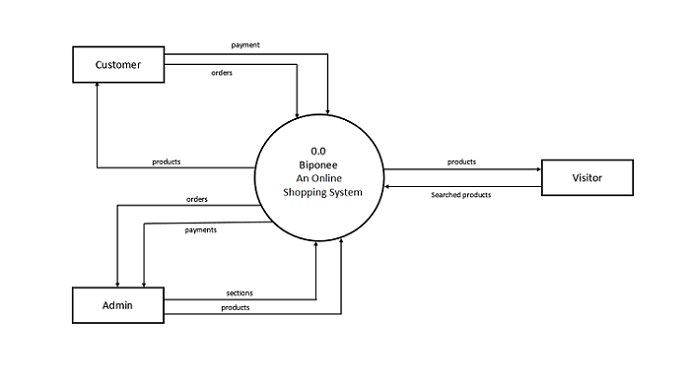
\includegraphics{figures/level0final.png}
\caption{Context Level DFD of Biponee}
\end{figure}

\newpage

\subsection{level 1 DFD}
 \begin{figure}
 \centering
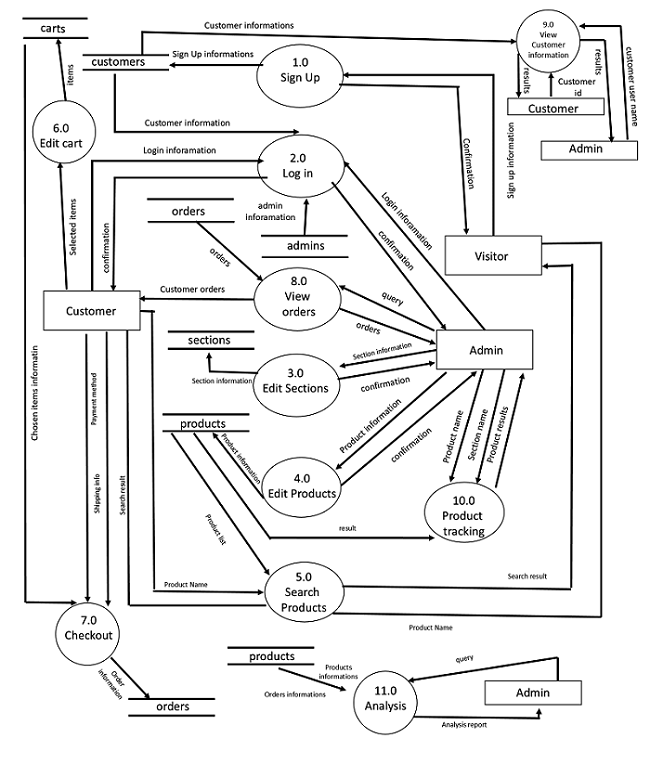
\includegraphics{figures/1s.png}
\caption{Level 1 DFD of Biponee}
\end{figure}


\newpage

\subsection{ Level 2 DFD }
 \begin{figure}
 \centering
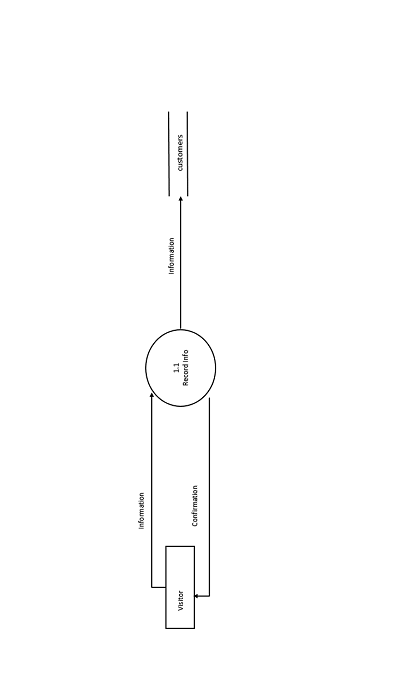
\includegraphics{figures/1final.png}
\caption{Sub-processes of Sign Up}
\end{figure}






 \begin{figure}
 \centering
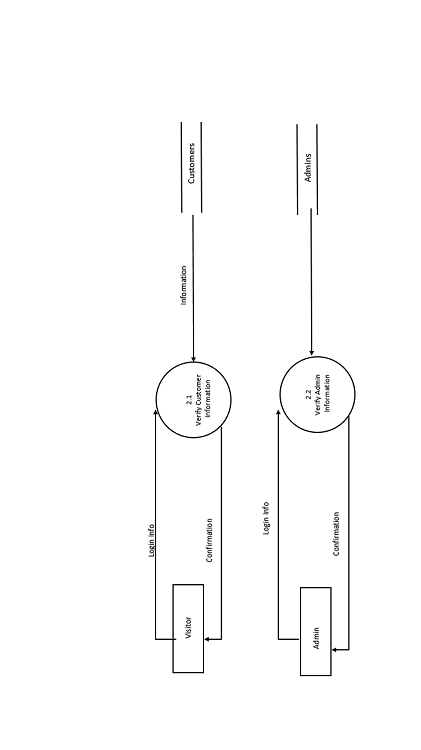
\includegraphics{figures/2final.png}
\caption{Sub-processes of Log in}
\end{figure}


 \begin{figure}
 \centering
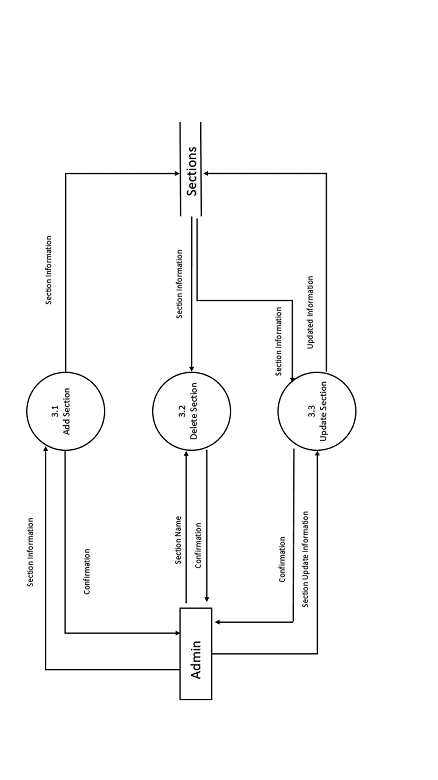
\includegraphics{figures/3final.png}
\caption{Sub-processes of Edit Sections}
\end{figure}



 \begin{figure}
 \centering
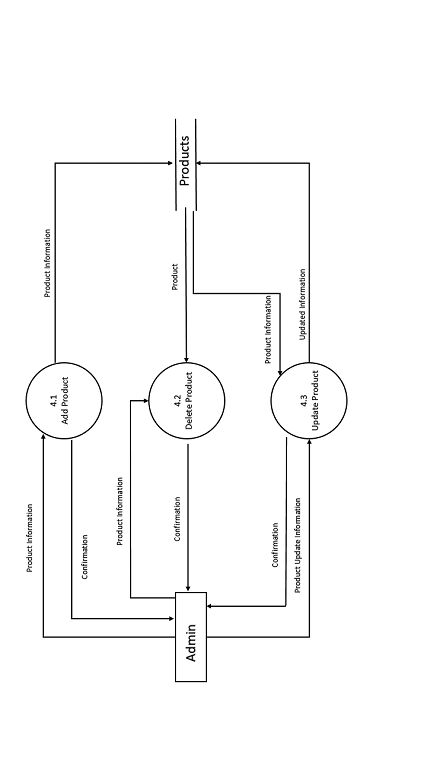
\includegraphics{figures/4final.png}
\caption{Sub-processes of Edit products}
\end{figure}



\begin{figure}
 \centering
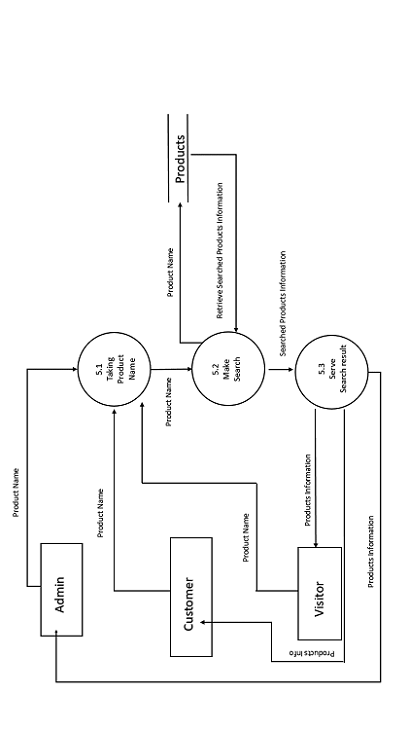
\includegraphics{figures/5final.png}
\caption{Sub-processes of Search Products}
\end{figure}




\begin{figure}
 \centering
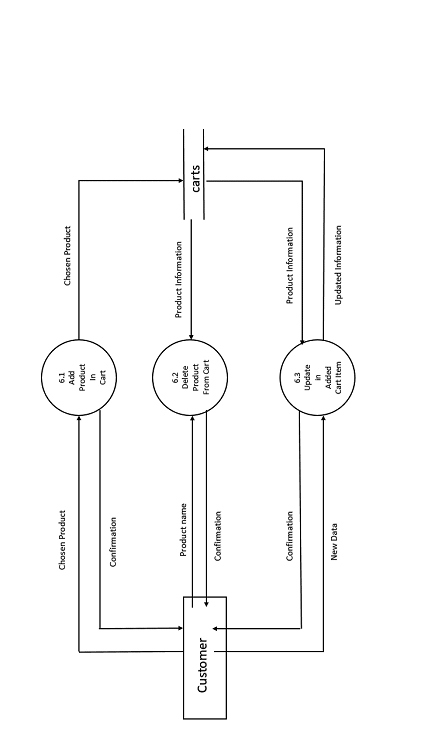
\includegraphics{figures/6final.png}
\caption{Sub-processes of  Edit cart}
\end{figure}


\begin{figure}
 \centering
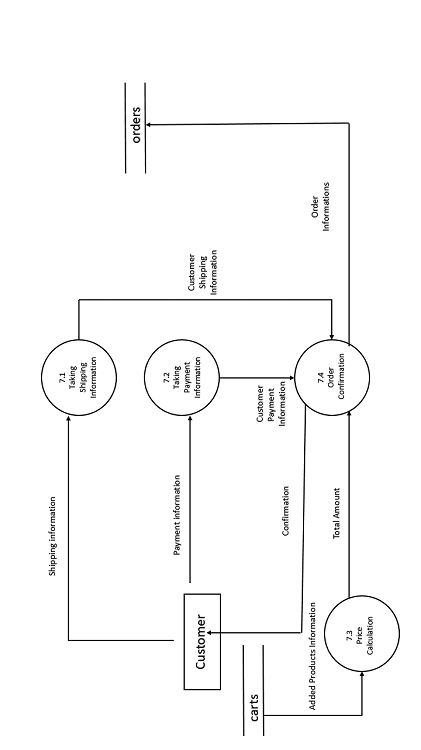
\includegraphics{figures/7final.png}
\caption{Sub-processes of  Order confirmation}
\end{figure}

\begin{figure}
 \centering
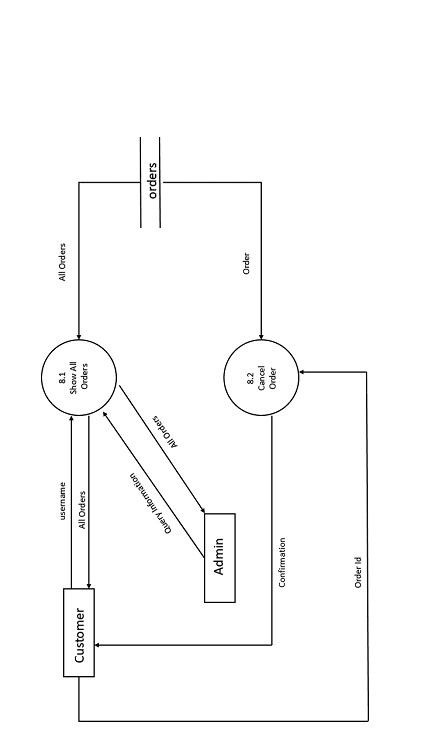
\includegraphics{figures/8final.png}
\caption{Sub-processes of View orders}
\end{figure}



\begin{figure}
 \centering
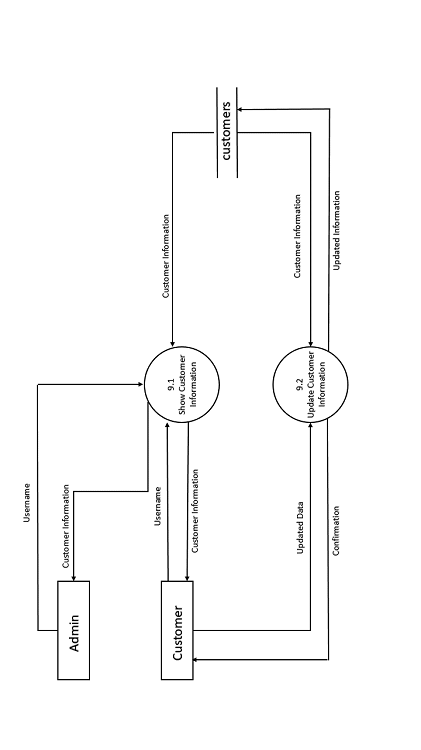
\includegraphics{figures/9final.png}
\caption{Sub-processes of View Customer information}
\end{figure}




\begin{figure}
 \centering
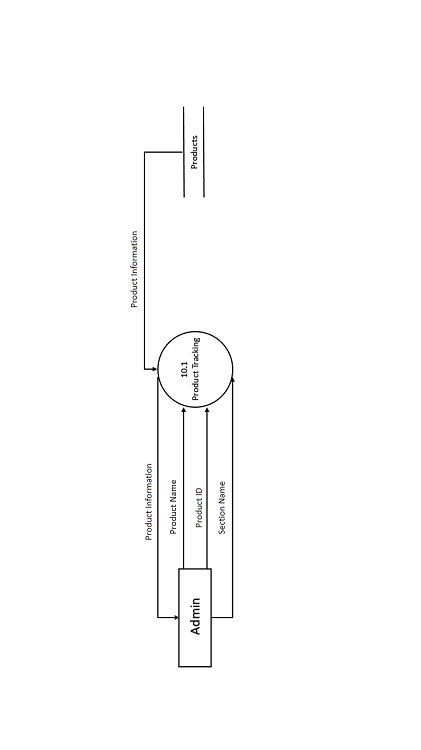
\includegraphics{figures/10final.png}
\caption{Sub-processes of Product tracking}
\end{figure}



\begin{figure}
 \centering
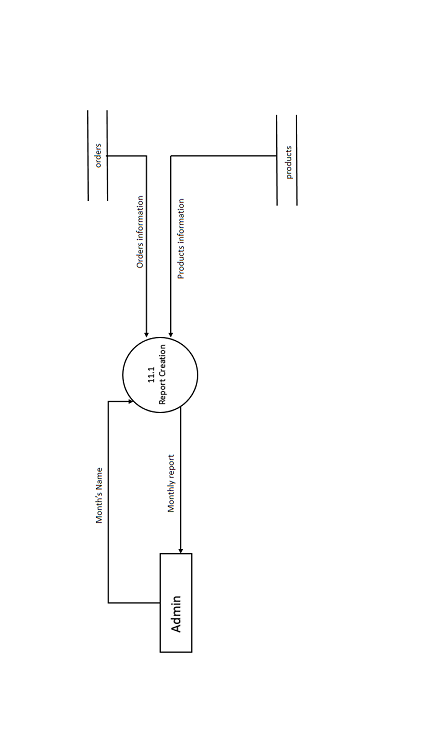
\includegraphics{figures/11final.png}
\caption{Sub-processes of Analysis}
\end{figure}

\newpage
\section{ Use Case Diagram}
 A use case diagram at its simplest is a representation of a user's interaction with the system that shows the relationship between the user and the different use cases in which the user is involved.
 
 \subsection{Actors}
  An actor specifies a role played by a user or any other system that interacts with the subject.\\ 
  The list of actors used by us:
\begin{itemize}
  \item Customer
  \item Visitor
    \item Admin
  \item Biponee Website
\end{itemize}


\subsection{Use Cases}
Use case is the sequence of actions that the system performs that yields an
observable result of value to an actor.
\begin{itemize}
  \item Sign up
  \item Login
    \item Browse sections
  \item Add to cart
    \item Checkout
  \item Edit sections
    \item Edit products
    \item View orders
    \item View customer informations
    \item Product tracking
    \item Analysis
    \item Confirmation
    \item Verify password
    \item Display login error
    \item Total calculation
    \item Update sections table
    \item Update products table
    \item Report calculations
 
\end{itemize}


\newpage
\subsection{Details of Use Case Models}

 \begin{figure}
\centering

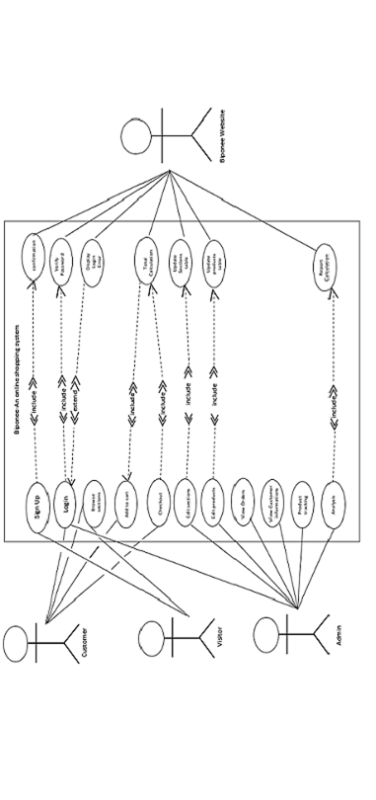
\includegraphics{figures/usecasenewv.png}

\caption{Use Case Diagram of Biponee}
\end{figure}


\newpage
\subsection{Conclusion}
 \begin{itemize}
    A Data flow diagram shows what kind of information will be input to and output from the system, how the data will advance through the system, and where the data will be stored. It does not show informations about process timing. From the DFD we can gather the clear concept of data flow of our project.\\
    \\
    
    We also draw the use case diagram of Biponee. we identify the actors and the use cases of our project from the diagram. We also identify how actually the actors communicate with the use cases from this diagram.\\
    \\
    
    We hope this use case diagram and data flow diagram concept will help us for develop Biponee
    efficiently.\\
     
 \end{itemize}
